\chapter*{Приложение А}
\addcontentsline{toc}{chapter}{Приложение А}
\renewcommand\thefigure{А.\arabic{figure}}  
\setcounter{figure}{0}
Приложение А содержит диаграмму классов разрабатываемого программного обеспечения.
\begin{figure}[H]
	\center{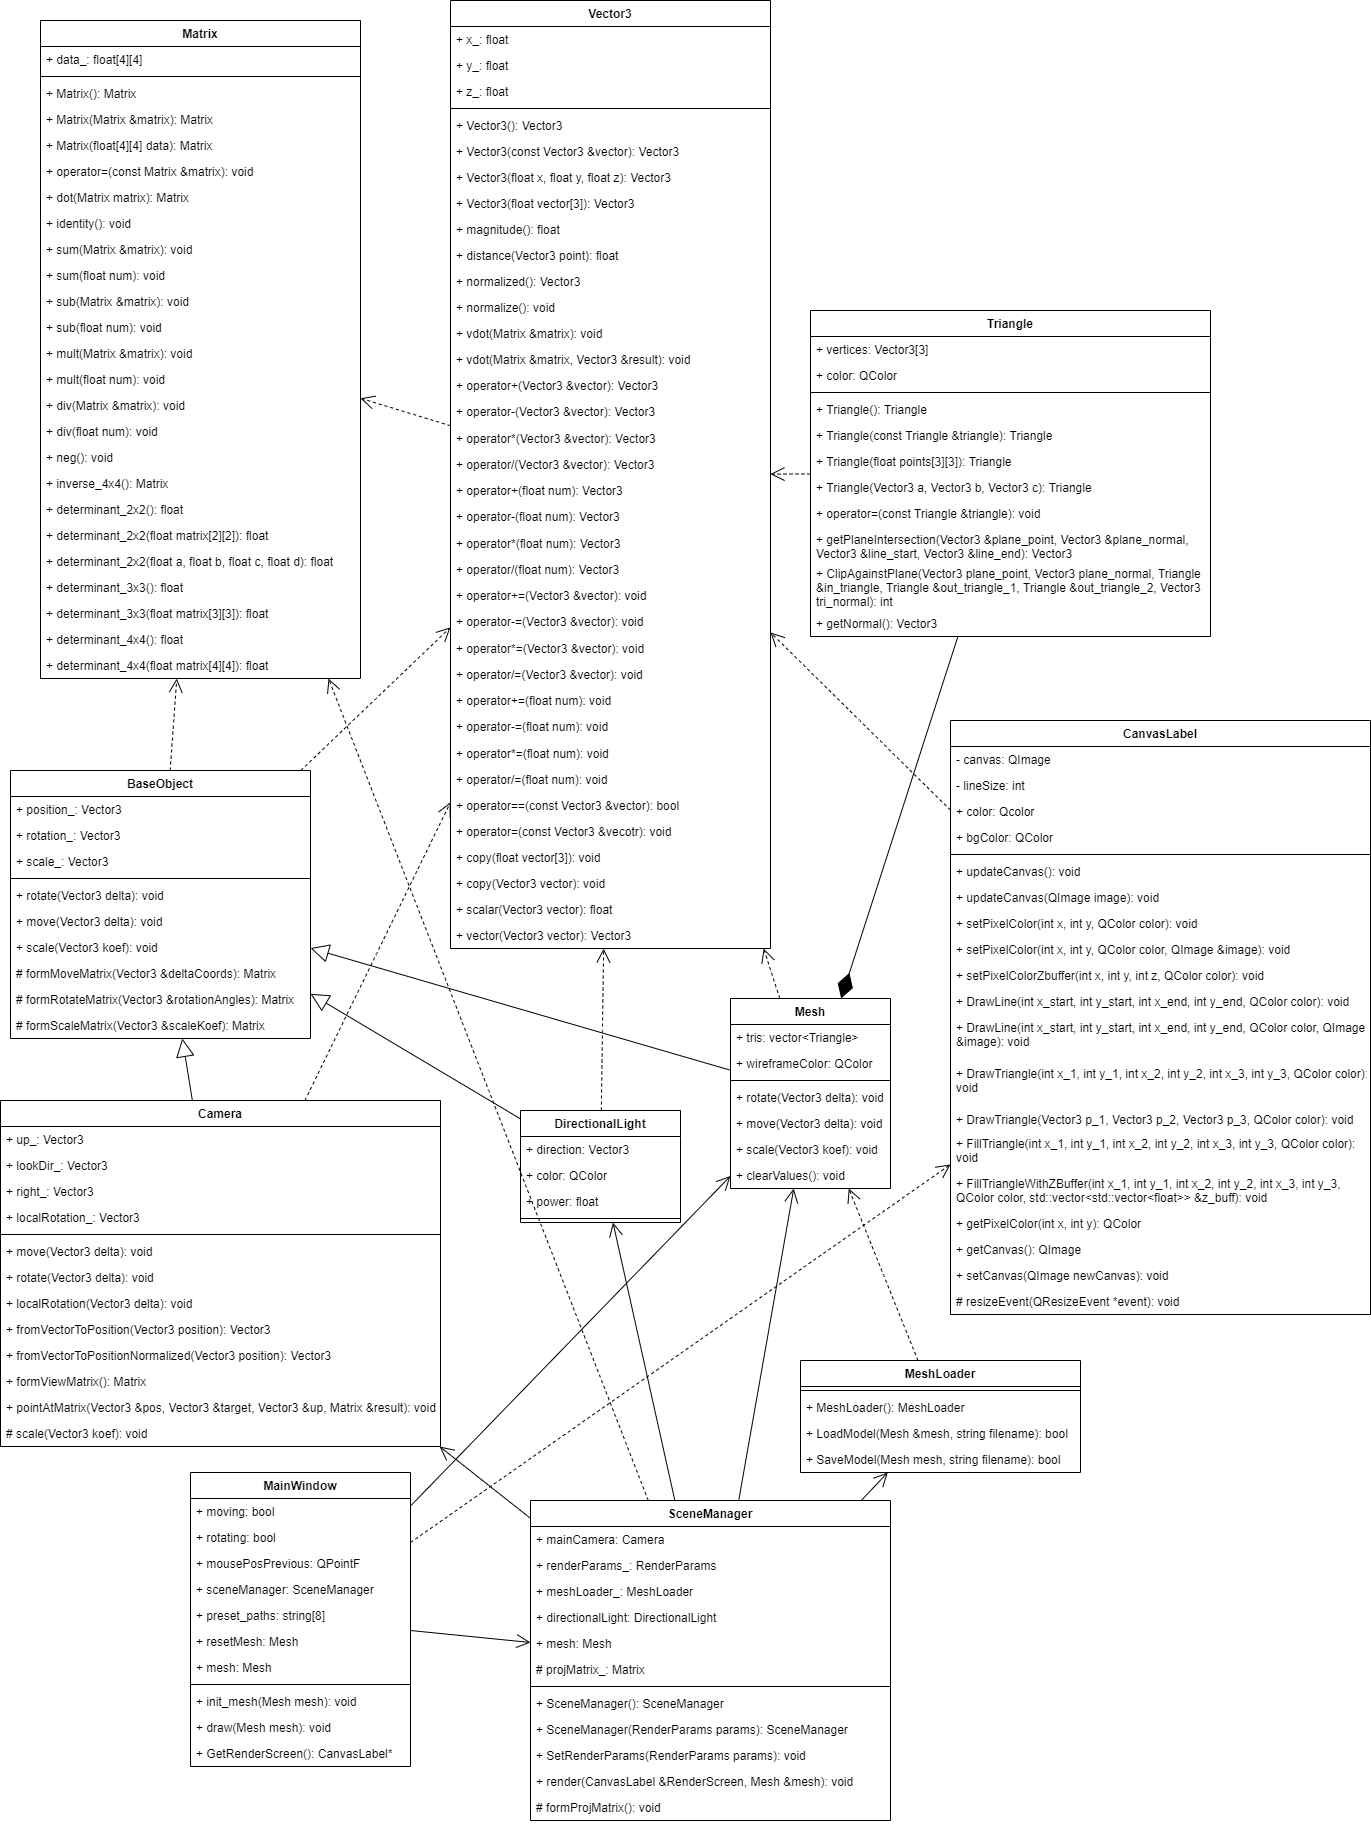
\includegraphics[scale=0.25]{classes}}
	\caption{Диаграмма классов разрабатываемого программного обеспечения}
	\label{fig:classes}
\end{figure}


\chapter*{Приложение Б}
\addcontentsline{toc}{chapter}{Приложение Б}
\renewcommand\thefigure{Б.\arabic{figure}}  
\setcounter{figure}{0}
Приложение Б содержит схему архитектуры разработанной нейронной сети.
\begin{figure}[H]
	\center{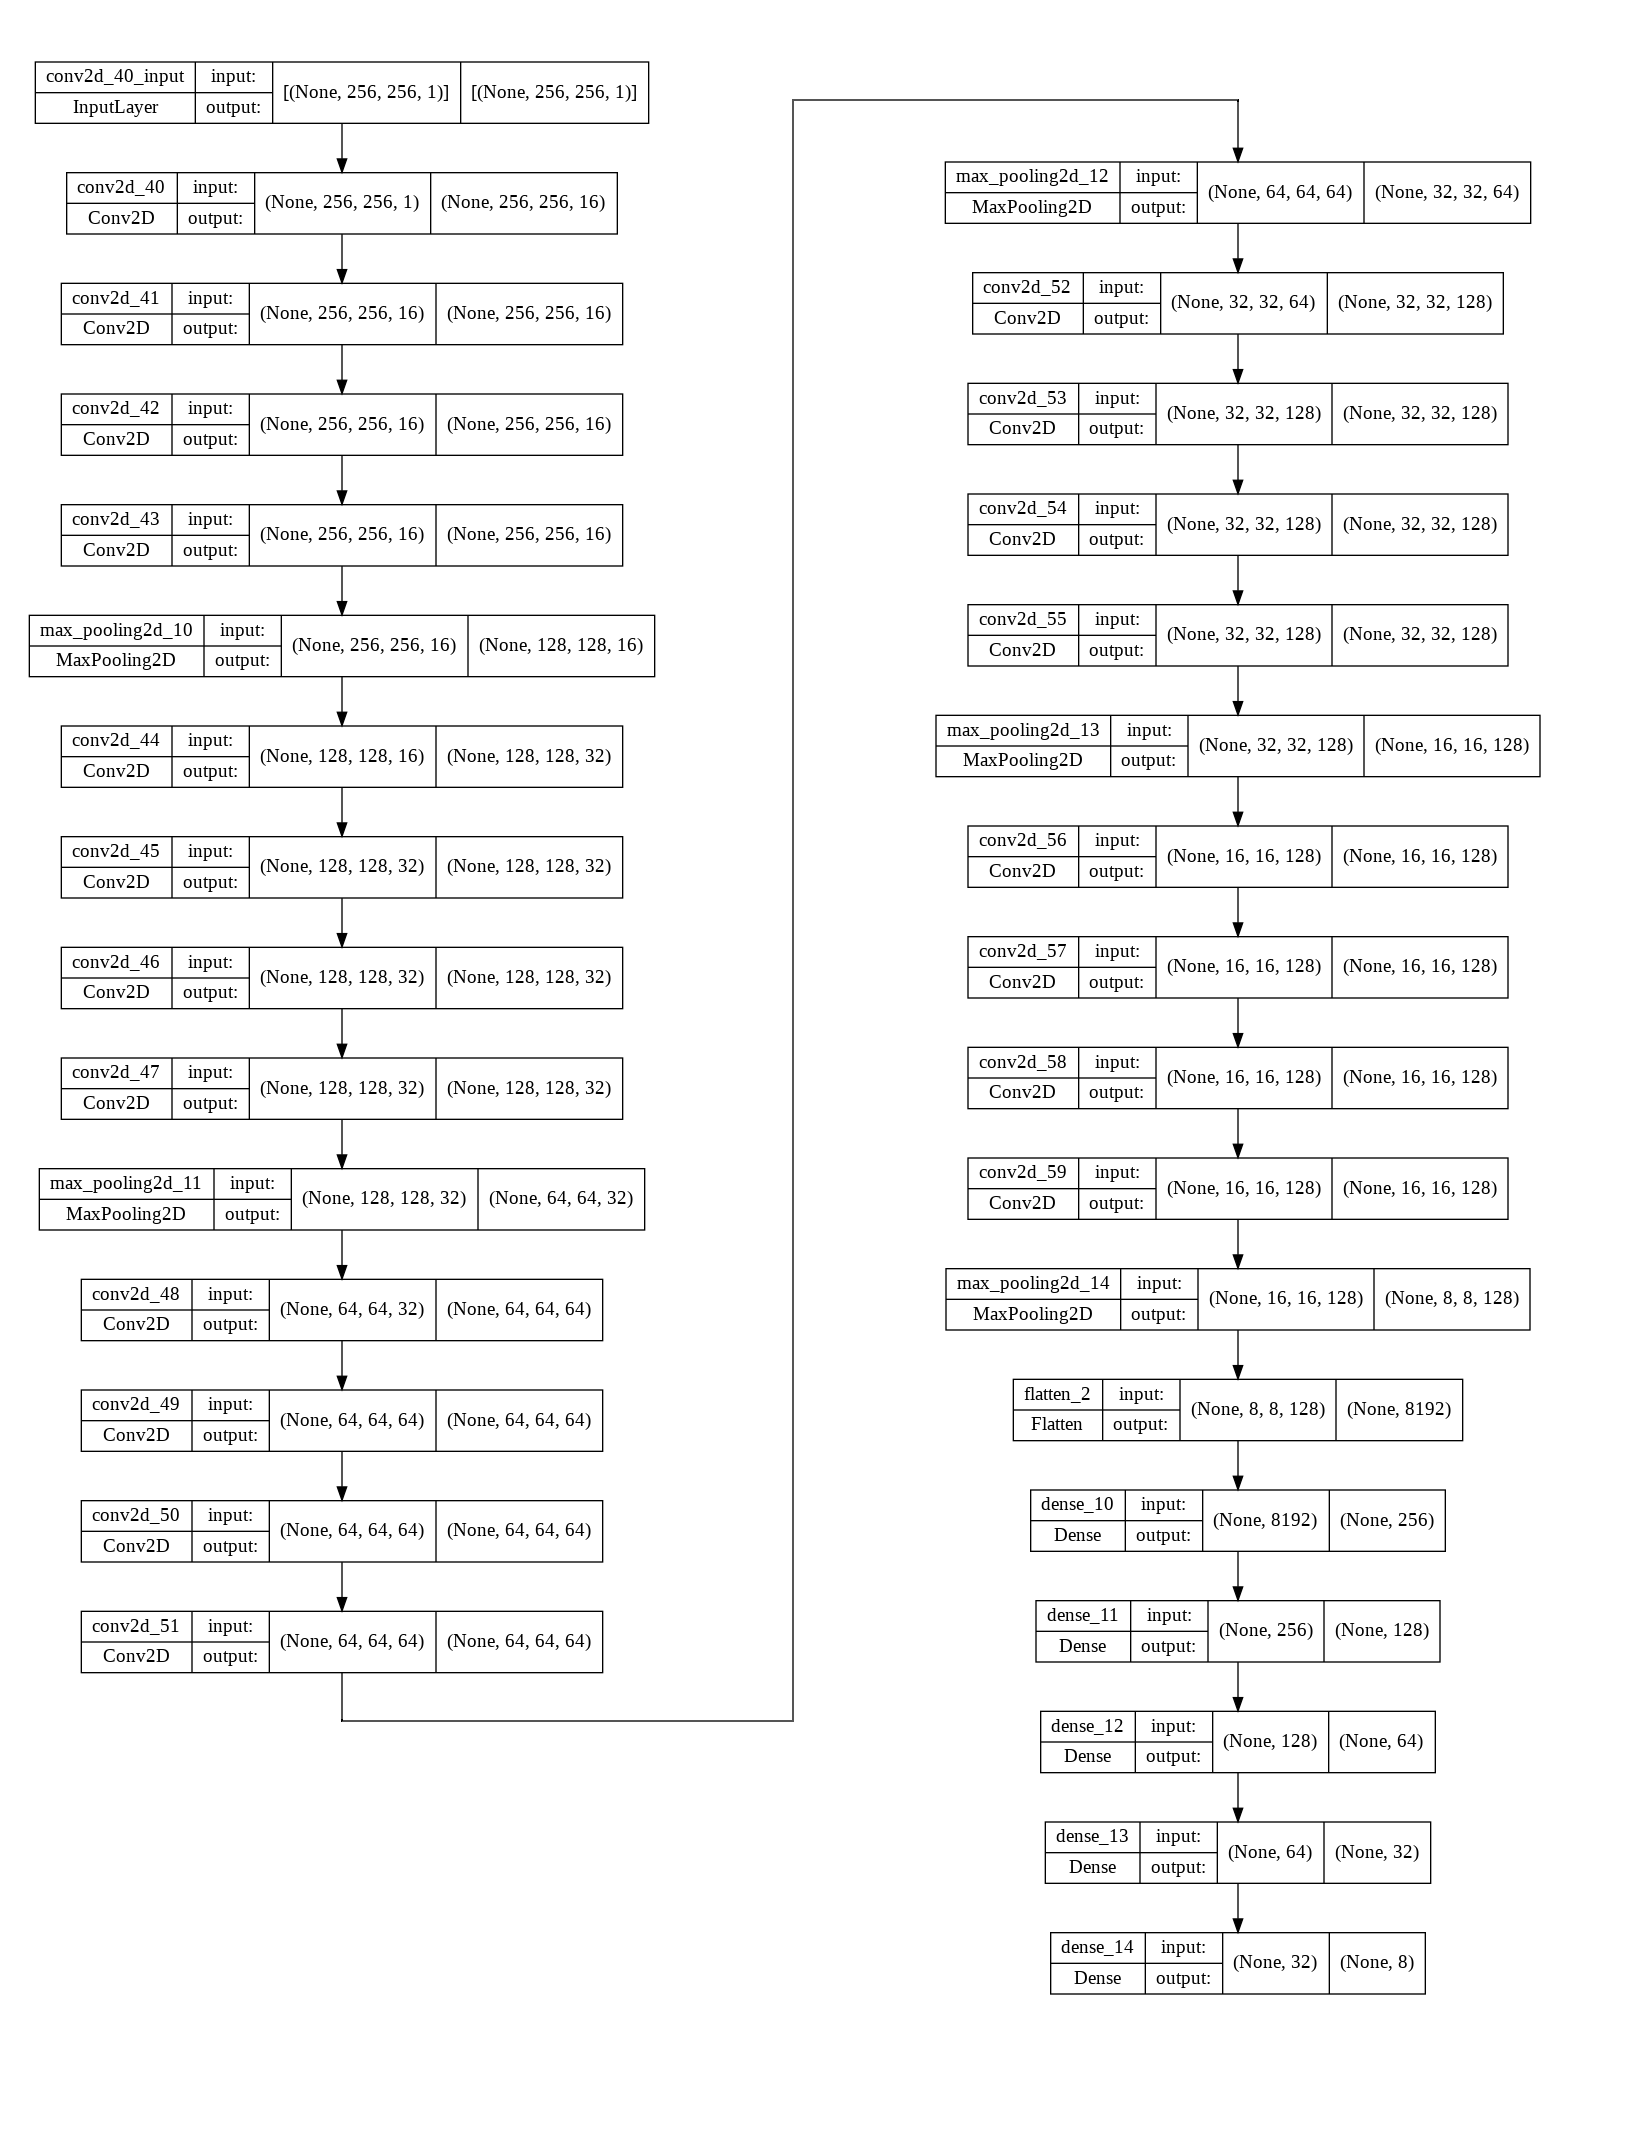
\includegraphics[scale=0.35]{model_img.png}}
	\caption{Схема архитектуры разработанной нейронной сети}
	\label{fig:cnn}
\end{figure}

\chapter*{Приложение В}
\addcontentsline{toc}{chapter}{Приложение В}
\renewcommand\thefigure{В.\arabic{figure}}  
\setcounter{figure}{0}
Приложение В содержит схему алгоритма z-буфера.
\begin{figure}[H]
	\center{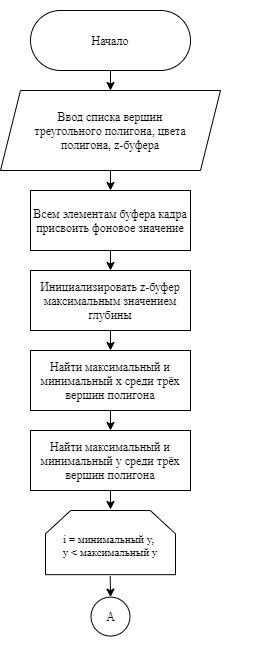
\includegraphics[scale=1.0]{z_buf_p_1}}
	\caption{Первая часть схемы алгоритма z-буфера}
	\label{fig:z_buf_1}
\end{figure}

\begin{figure}[H]
	\center{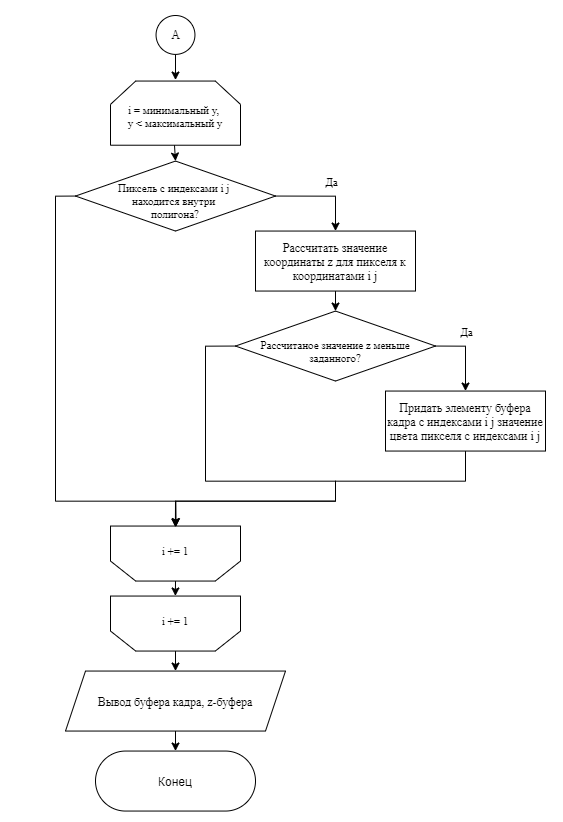
\includegraphics[scale=1.0]{z_buf_p_2}}
	\caption{Вторая часть схемы алгоритма z-буфера}
	\label{fig:z_buf_2}
\end{figure}


\chapter*{Приложение Г}
\addcontentsline{toc}{chapter}{Приложение Г}
\renewcommand\thelstlisting{Г.\arabic{lstlisting}}  
\setcounter{lstlisting}{0}
Приложение В содержит листинги реализаций основных алгоритмов.

Ниже в листинге \ref{lst:render} представлена реализация общего алгоритма отрисовки.

\begin{lstlisting}[caption = Реализация общего алгоритма отрисовки, label = lst:render]
void SceneManager::render(CanvasLabel &RenderScreen, Mesh &mesh)
{
    Matrix viewMatrix;
    viewMatrix = mainCamera.formViewMatrix();

    std::vector<std::vector<float>> z_buff(RenderScreen.size().height(), std::vector<float>(RenderScreen.size().width()));

    for (auto &row : z_buff)
    {
        for (auto &elem : row)
        {
           elem = std::numeric_limits<float>::max();
        }
    }

    vector<Triangle> vecTrianglesToRaster;

    for (auto &tri : mesh.tris)
    {
        vecTrianglesToRaster.clear();

        float dp = directionalLight.direction.normalized().scalar(tri.getNormal());

        QColor color;
        if (dp <= 0)
        {
            color.setRgb(0, 0, 0);
        }
        else
        {
            int colorVal = dp * 255 * directionalLight.power;
            if (colorVal > 255)
                colorVal = 255;
            color.setRgb(colorVal, colorVal, colorVal);
        }
        tri.color = color;

        Triangle triangleProjected, triangleViewed;

        tri.vertices[0].vdot(viewMatrix, triangleViewed.vertices[0]);
        tri.vertices[1].vdot(viewMatrix, triangleViewed.vertices[1]);
        tri.vertices[2].vdot(viewMatrix, triangleViewed.vertices[2]);

        int clipped_num;
        Triangle clipped[2];
        clipped_num = triangleViewed.ClipAgainstPlane({0.0f, 0.0f, renderParams_.fNear}, {0.0f, 0.0f, 1.0f}, triangleViewed, clipped[0], clipped[1], triangleViewed.getNormal());

        for (int n = 0; n < clipped_num; n++)
        {
            clipped[n].vertices[0].vdot(projMatrix_, triangleProjected.vertices[0]);
            clipped[n].vertices[1].vdot(projMatrix_, triangleProjected.vertices[1]);
            clipped[n].vertices[2].vdot(projMatrix_, triangleProjected.vertices[2]);

            triangleProjected.vertices[0].z_ = clipped[n].vertices[0].z_;
            triangleProjected.vertices[1].z_ = clipped[n].vertices[1].z_;
            triangleProjected.vertices[2].z_ = clipped[n].vertices[2].z_;

            vecTrianglesToRaster.push_back(triangleProjected);
        }

        for (auto &triToRaster : vecTrianglesToRaster)
        {
            triToRaster.vertices[0].x_ *= 0.1 * RenderScreen.size().width();
            triToRaster.vertices[0].y_ *= 0.1 * RenderScreen.size().height();

            triToRaster.vertices[1].x_ *= 0.1 * RenderScreen.size().width();
            triToRaster.vertices[1].y_ *= 0.1 * RenderScreen.size().height();

            triToRaster.vertices[2].x_ *= 0.1 * RenderScreen.size().width();
            triToRaster.vertices[2].y_ *= 0.1 * RenderScreen.size().height();

            Triangle clipped[2];
            Triangle test_temp;
            list<Triangle> listTriangles;

            listTriangles.push_back(triToRaster);
            int nNewTriangles = 1;


            for (int p = 0; p < 4; p++)
            {
                int nTrisToAdd = 0;
                while (nNewTriangles > 0)
                {
                    Triangle test = listTriangles.front();
                    listTriangles.pop_front();
                    nNewTriangles--;
                    switch (p)
                    {
                    case 0:
                        nTrisToAdd = test_temp.ClipAgainstPlane({ 0.0f, (float)RenderScreen.height()/2 - 1, 0.0f }, { 0.0f, -1.0f, 0.0f }, test, clipped[0], clipped[1], test.getNormal());
                        break;
                    case 1:
                        nTrisToAdd = test_temp.ClipAgainstPlane({ 0.0f, -(float)RenderScreen.height()/2 + 1, 0.0f }, { 0.0f, 1.0f, 0.0f }, test, clipped[0], clipped[1], test.getNormal());
                        break;
                    case 2:
                        nTrisToAdd = test_temp.ClipAgainstPlane({ (float)RenderScreen.width()/2 - 1, 0.0f, 0.0f }, { -1.0f, 0.0f, 0.0f }, test, clipped[0], clipped[1], test.getNormal());
                        break;
                    case 3:
                        nTrisToAdd = test_temp.ClipAgainstPlane({ -(float)RenderScreen.width()/2 + 1, 0.0f, 0.0f }, { 1.0f, 0.0f, 0.0f }, test, clipped[0], clipped[1], test.getNormal());
                        break;
                    }

                    for (int w = 0; w < nTrisToAdd; w++)
                        listTriangles.push_back(clipped[w]);

                }
                nNewTriangles = listTriangles.size();
            }


            for (auto &tris : listTriangles)
            {
                RenderScreen.FillTriangleWithZBuffer(
                    tris.vertices[0],
                    tris.vertices[1],
                    tris.vertices[2],
                    tri.color,
                    z_buff
                 );
            }
        }
    }

    RenderScreen.updateCanvas();
}
\end{lstlisting}

Ниже в листинге \ref{lst:clip} представлена реализация алгоритма отсекания невидимой части треугольного полигона.

\begin{lstlisting}[caption = Реализация общего алгоритма отрисовки, label = lst:clip]
int Triangle::ClipAgainstPlane(Vector3 plane_point, Vector3 plane_normal, Triangle &in_triangle, Triangle &out_triangle_1, Triangle &out_triangle_2, Vector3 tri_normal)
{
    plane_normal = plane_normal.normalized();
    tri_normal.normalize();
    auto dist = [&](Vector3 p)
    {
        return (plane_normal.x_ * p.x_ + plane_normal.y_ * p.y_ + plane_normal.z_ * p.z_ - plane_normal.scalar(plane_point));
    };

    Vector3* inside_points[3];
    int nInsidePointCount = 0;
    Vector3* outside_points[3];
    int nOutsidePointCount = 0;

    float d0 = dist(in_triangle.vertices[0]);
    float d1 = dist(in_triangle.vertices[1]);
    float d2 = dist(in_triangle.vertices[2]);

    if (d0 >= 0)
        inside_points[nInsidePointCount++] = &in_triangle.vertices[0];
    else
        outside_points[nOutsidePointCount++] = &in_triangle.vertices[0];

    if (d1 >= 0)
        inside_points[nInsidePointCount++] = &in_triangle.vertices[1];
    else
        outside_points[nOutsidePointCount++] = &in_triangle.vertices[1];

    if (d2 >= 0)
        inside_points[nInsidePointCount++] = &in_triangle.vertices[2];
    else
        outside_points[nOutsidePointCount++] = &in_triangle.vertices[2];

    if (nInsidePointCount == 0)
        return 0;

    if (nInsidePointCount == 3)
    {
        out_triangle_1 = in_triangle;

        if (out_triangle_1.getNormal().normalized().scalar(tri_normal) < 0)
        {
            Vector3 temp = out_triangle_1.vertices[2];
            out_triangle_1.vertices[2] = out_triangle_1.vertices[1];
            out_triangle_1.vertices[1] = temp;
        }
        return 1;
    }

    if (nInsidePointCount == 1 && nOutsidePointCount == 2)
    {
        out_triangle_1 = in_triangle;
        out_triangle_1.vertices[0] = *inside_points[0];
        out_triangle_1.vertices[1] = getPlaneIntersection(plane_point, plane_normal, *inside_points[0], *outside_points[0]);
        out_triangle_1.vertices[2] = getPlaneIntersection(plane_point, plane_normal, *inside_points[0], *outside_points[1]);

        if (out_triangle_1.getNormal().normalized().scalar(tri_normal) < 0)
        {
            Vector3 temp = out_triangle_1.vertices[2];
            out_triangle_1.vertices[2] = out_triangle_1.vertices[1];
            out_triangle_1.vertices[1] = temp;
        }

        return 1;
    }

    if (nInsidePointCount == 2 && nOutsidePointCount == 1)
    {
        out_triangle_1 = in_triangle;
        out_triangle_2 = in_triangle;

        out_triangle_1.vertices[0] = *inside_points[0];
        out_triangle_1.vertices[1] = *inside_points[1];
        out_triangle_1.vertices[2] = getPlaneIntersection(plane_point, plane_normal, *inside_points[0], *outside_points[0]);

        if (out_triangle_1.getNormal().normalized().scalar(tri_normal) < 0)
        {
            Vector3 temp = out_triangle_1.vertices[2];
            out_triangle_1.vertices[2] = out_triangle_1.vertices[1];
            out_triangle_1.vertices[1] = temp;
        }

        out_triangle_2.vertices[0] = *inside_points[1];
        out_triangle_2.vertices[1] = out_triangle_1.vertices[2];
        if (abs(out_triangle_2.vertices[1].x_ - out_triangle_2.vertices[0].x_) < 0.0001 &&\
            abs(out_triangle_2.vertices[1].y_ - out_triangle_2.vertices[0].y_) < 0.0001 &&\
            abs(out_triangle_2.vertices[1].z_ - out_triangle_2.vertices[0].z_) < 0.0001)
            out_triangle_2.vertices[1] = out_triangle_1.vertices[1];
        out_triangle_2.vertices[2] = getPlaneIntersection(plane_point, plane_normal, *inside_points[1], *outside_points[0]);

        if (out_triangle_2.getNormal().normalized().scalar(tri_normal) < 0)
        {
            Vector3 temp = out_triangle_2.vertices[2];
            out_triangle_2.vertices[2] = out_triangle_2.vertices[1];
            out_triangle_2.vertices[1] = temp;
        }

        return 2;
    }
    return 0;
}
\end{lstlisting}

Ниже в листинге \ref{lst:zbuf} представлена реализация алгоритма z-буфера.

\begin{lstlisting}[caption = Реализация общего алгоритма отрисовки, label = lst:zbuf]
void CanvasLabel::FillTriangleWithZBuffer(Vector3 p_1, Vector3 p_2, Vector3 p_3, QColor color, std::vector<std::vector<float>> &z_buff)
{
    int x_max = get_max(p_1.x_, p_2.x_, p_3.x_);
    int y_max = get_max(p_1.y_, p_2.y_, p_3.y_);

    int x_min = get_min(p_1.x_, p_2.x_, p_3.x_);
    int y_min = get_min(p_1.y_, p_2.y_, p_3.y_);

    Vector3 temp_p_1;
    Vector3 temp_p_2;
    Vector3 temp_p_3;

    temp_p_1.y_ = y_max;
    if (int(temp_p_1.y_) == int(p_1.y_))
        temp_p_1 = p_1;
    if (int(temp_p_1.y_) == int(p_2.y_))
        temp_p_1 = p_2;
    if (int(temp_p_1.y_) == int(p_3.y_))
        temp_p_1 = p_3;

    temp_p_3.y_ = y_min;
    if (int(temp_p_3.y_) == int(p_1.y_) && int(temp_p_1.y_) != int(p_1.y_))
        temp_p_3 = p_1;
    if (int(temp_p_3.y_) == int(p_2.y_) && int(temp_p_1.y_) != int(p_2.y_))
        temp_p_3 = p_2;
    if (int(temp_p_3.y_) == int(p_3.y_) && int(temp_p_1.y_) != int(p_3.y_))
        temp_p_3 = p_3;

    if ((temp_p_1 == p_1 && temp_p_3 == p_2) || (temp_p_1 == p_2 && temp_p_3 == p_1))
        temp_p_2 = p_3;
    if ((temp_p_1 == p_1 && temp_p_3 == p_3) || (temp_p_1 == p_3 && temp_p_3 == p_1))
        temp_p_2 = p_2;
    if ((temp_p_1 == p_2 && temp_p_3 == p_3) || (temp_p_1 == p_3 && temp_p_3 == p_2))
        temp_p_2 = p_1;

    for (int y = y_min; y < y_max; y++)
    {
        for (int x = x_min; x < x_max; x++)
        {
            if (abs(x) < this->size().width()/2 && abs(y) < this->size().height()/2)
            {
                float e21 = TestPoint(x, y, p_2.x_, p_2.y_, p_1.x_, p_1.y_);
                float e32 = TestPoint(x, y, p_3.x_, p_3.y_, p_2.x_, p_2.y_);
                float e13 = TestPoint(x, y, p_1.x_, p_1.y_, p_3.x_, p_3.y_);

                if (e21 >= 0.0f && e32 >= 0.0f && e13 >= 0.0f)
                {
                    if (y == y_max || y == y_min)
                    {
                        if ((y == int(temp_p_2.y_) && (y == int(temp_p_1.y_))))
                        {
                            float z = temp_p_1.z_ + (temp_p_2.z_ - temp_p_1.z_) * ((x - temp_p_1.x_)/(temp_p_2.x_ - temp_p_1.x_));
                            if (z < z_buff[this->size().height()/2 - y][x + this->size().width()/2])
                            {
                                setPixelColor(x, y, color);
                                z_buff[this->size().height()/2 - y][x + this->size().width()/2] = z;
                            }
                            //setPixelColor(x, y, color);
                        }
                        else if ((y == int(temp_p_2.y_) && (y == int(temp_p_3.y_))))
                        {
                            float z = temp_p_3.z_ + (temp_p_2.z_ - temp_p_3.z_) * ((x - temp_p_3.x_)/(temp_p_2.x_ - temp_p_3.x_));
                            if (z < z_buff[this->size().height()/2 - y][x + this->size().width()/2])
                            {
                                setPixelColor(x, y, color);
                                z_buff[this->size().height()/2 - y][x + this->size().width()/2] = z;
                            }
                            //setPixelColor(x, y, color);
                        }
                        else if (y == int(temp_p_1.y_))
                        {
                            float z = temp_p_1.z_;
                            if (z < z_buff[this->size().height()/2 - y][x + this->size().width()/2])
                            {
                                setPixelColor(x, y, color);
                                z_buff[this->size().height()/2 - y][x + this->size().width()/2] = z;
                            }
                            //setPixelColor(x, y, color);
                        }
                        else if (y == int(temp_p_3.y_))
                        {
                            float z = temp_p_3.z_;
                            if (z < z_buff[this->size().height()/2 - y][x + this->size().width()/2])
                            {
                                setPixelColor(x, y, color);
                                z_buff[this->size().height()/2 - y][x + this->size().width()/2] = z;
                            }
                            //setPixelColor(x, y, color);
                        }
                    }
                    else if (y >= int(temp_p_2.y_))
                    {
                        int x_a = temp_p_1.x_ + (temp_p_2.x_ - temp_p_1.x_)*((y - temp_p_1.y_)/(temp_p_2.y_ - temp_p_1.y_));
                        int x_b = temp_p_1.x_ + (temp_p_3.x_ - temp_p_1.x_)*((y - temp_p_1.y_)/(temp_p_3.y_ - temp_p_1.y_));
                        float z_a = temp_p_1.z_ + (temp_p_2.z_ - temp_p_1.z_)*((y - temp_p_1.y_)/(temp_p_2.y_ - temp_p_1.y_));
                        float z_b = temp_p_1.z_ + (temp_p_3.z_ - temp_p_1.z_)*((y - temp_p_1.y_)/(temp_p_3.y_ - temp_p_1.y_));

                        if (x_a != x_b)
                        {
                            float z = z_a + (z_b - z_a)*((x - x_a)/(x_b - x_a));

                            if (z < z_buff[this->size().height()/2 - y][x + this->size().width()/2])
                            {
                                setPixelColor(x, y, color);
                                z_buff[this->size().height()/2 - y][x + this->size().width()/2] = z;
                            }
                        }
                        else
                        {
                            if (z_a < z_buff[this->size().height()/2 - y][x + this->size().width()/2])
                            {
                                setPixelColor(x, y, color);
                                z_buff[this->size().height()/2 - y][x + this->size().width()/2] = z_a;
                            }
                        }
                    }
                    else if (y < int(temp_p_2.y_))
                    {
                        int x_a = temp_p_2.x_ + (temp_p_3.x_ - temp_p_2.x_)*((y - temp_p_2.y_)/(temp_p_3.y_ - temp_p_2.y_));
                        int x_b = temp_p_1.x_ + (temp_p_3.x_ - temp_p_1.x_)*((y - temp_p_1.y_)/(temp_p_3.y_ - temp_p_1.y_));
                        float z_a = temp_p_2.z_ + (temp_p_3.z_ - temp_p_2.z_)*((y - temp_p_2.y_)/(temp_p_3.y_ - temp_p_2.y_));
                        float z_b = temp_p_1.z_ + (temp_p_3.z_ - temp_p_1.z_)*((y - temp_p_1.y_)/(temp_p_3.y_ - temp_p_1.y_));

                        if (x_a != x_b)
                        {
                            float z = z_a + (z_b - z_a)*((x - x_a)/(x_b - x_a));

                            if (z < z_buff[this->size().height()/2 - y][x + this->size().width()/2])
                            {
                                setPixelColor(x, y, color);
                                z_buff[this->size().height()/2 - y][x + this->size().width()/2] = z;
                            }
                            //setPixelColor(x, y, color);
                        }
                        else
                        {
                            if (z_a < z_buff[this->size().height()/2 - y][x + this->size().width()/2])
                            {
                                setPixelColor(x, y, color);
                                z_buff[this->size().height()/2 - y][x + this->size().width()/2] = z_a;
                            }
                        }
                    }
                }
            }
        }
    }
}
\end{lstlisting}

Ниже в листинге \ref{lst:learn} представлена реализация алгоритма обучения свёрточной нейросети.

\begin{lstlisting}[caption = Реализация алгоритма обучения свёрточной нейросети, label = lst:learn]
import tensorflow as tf
from tensorflow import keras
from keras import layers
import numpy as np
import cv2

train_materials_path = "D:/Storage/Andrew/BMSTU/BMSTU/CW/Work/CourseProject/TrainMaterials/"

import os, os.path

x_train = []
y_train = []

#size of dataset
dataset_size = len(os.listdir(train_materials_path))
classes = 8
image_size = (256, 256)
image_shape = (256, 256, 1)
batch_size = 128

import os

clahe = cv2.createCLAHE(clipLimit=2.0, tileGridSize=(8,8))
count = 0

for name in os.listdir(train_materials_path):
  fpath_img = train_materials_path + name
  image = cv2.imread(fpath_img, cv2.IMREAD_GRAYSCALE)
  
  min_dim = min(image.shape)
  w = min_dim
  h = min_dim
  center = image.shape
  x = center[1]/2 - w/2
  y = center[0]/2 - h/2

  crop_img = image[int(y):int(y+h), int(x):int(x+w)]

  img_clh = clahe.apply(crop_img)
  new_img = cv2.resize(img_clh, image_size)

  x_train.append(new_img)

  index = int(name.split('_')[1])
  res_vec = [0] * classes
  res_vec[index] = 1
  
  y_train.append(res_vec)
  count += 1
  if count \% 100 == 0:
    os.system('cls')
    print(count, ':', dataset_size)

x_train = np.array(x_train)
y_train = np.array(y_train)    

from keras.layers.pooling import MaxPooling2D
from keras import Sequential
from keras.layers import Conv2D, Flatten, Dense, MaxPool2D, AveragePooling2D, BatchNormalization

model = Sequential()

model.add(Conv2D(16, kernel_size=(9,9), strides=(1,1), padding='same', input_shape=image_shape))
model.add(Conv2D(16, kernel_size=(9,9), strides=(1,1), padding='same'))
model.add(Conv2D(16, kernel_size=(9,9), strides=(1,1), padding='same'))
model.add(Conv2D(16, kernel_size=(9,9), strides=(1,1), padding='same'))
model.add(MaxPooling2D(pool_size=(2,2)))

model.add(Conv2D(32, kernel_size=(7,7), strides=(1,1), padding='same'))
model.add(Conv2D(32, kernel_size=(7,7), strides=(1,1), padding='same'))
model.add(Conv2D(32, kernel_size=(7,7), strides=(1,1), padding='same'))
model.add(Conv2D(32, kernel_size=(7,7), strides=(1,1), padding='same'))
model.add(MaxPooling2D(pool_size=(2,2)))

model.add(Conv2D(64, kernel_size=(5,5), strides=(1,1), padding='same'))
model.add(Conv2D(64, kernel_size=(5,5), strides=(1,1), padding='same'))
model.add(Conv2D(64, kernel_size=(5,5), strides=(1,1), padding='same'))
model.add(Conv2D(64, kernel_size=(5,5), strides=(1,1), padding='same'))
model.add(MaxPooling2D(pool_size=(2,2)))

model.add(Conv2D(128, kernel_size=(3,3), strides=(1,1), padding='same'))
model.add(Conv2D(128, kernel_size=(3,3), strides=(1,1), padding='same'))
model.add(Conv2D(128, kernel_size=(3,3), strides=(1,1), padding='same'))
model.add(Conv2D(128, kernel_size=(3,3), strides=(1,1), padding='same'))
model.add(MaxPooling2D(pool_size=(2,2)))

model.add(Conv2D(128, kernel_size=(3,3), strides=(1,1), padding='same'))
model.add(Conv2D(128, kernel_size=(3,3), strides=(1,1), padding='same'))
model.add(Conv2D(128, kernel_size=(3,3), strides=(1,1), padding='same'))
model.add(Conv2D(128, kernel_size=(3,3), strides=(1,1), padding='same'))
model.add(MaxPooling2D(pool_size=(2,2)))

model.add(Flatten())

model.add(Dense(256, activation='relu'))
model.add(Dense(128, activation='relu'))
model.add(Dense(64, activation='relu'))
model.add(Dense(32, activation='relu'))
model.add(Dense(classes, activation='softmax'))

from keras import losses
from keras import metrics

epochs = 20

opt = tf.keras.optimizers.Adam(learning_rate=0.001, decay=1e-3 / 200)

callbacks = [
    keras.callbacks.ModelCheckpoint("save_model_at_{epoch}.h5"),
]
model.compile(loss=losses.categorical_crossentropy, optimizer=opt, metrics=metrics.Accuracy())

history = model.fit(
    x_train, y_train, epochs=epochs, callbacks=callbacks, validation_split=0.2,
)

model.save('new_model.h5')
\end{lstlisting}

Ниже в листинге \ref{lst:predict} представлена реализация общего алгоритма отрисовки.

\begin{lstlisting}[caption = Реализация алгоритма определения трёхмерного объекта\, наиболее вероятно являющимся объектом изображённым на снимке, label = lst:predict]
def predict_model(fpath_img: str) -> int:
    import cv2
    import numpy as np
    import keras
    import tensorflow as tf
    from keras import layers
    
    try:
        image_size = (256, 256)

        clahe = cv2.createCLAHE(clipLimit=2.0, tileGridSize=(8,8))
        image = cv2.imread(fpath_img, cv2.IMREAD_GRAYSCALE)
        
        max_index = 0
        count = 0
        max_val = 0

        min_dim = min(image.shape)
        w = min_dim
        h = min_dim
        center = image.shape
        x = center[1]/2 - w/2
        y = center[0]/2 - h/2

        crop_img = image[int(y):int(y+h), int(x):int(x+w)]

        img_clh = clahe.apply(crop_img)
        new_img = cv2.resize(img_clh, image_size)

        from keras.models import load_model
        import os
        dir_path = os.path.dirname(os.path.realpath(__file__))
        model = load_model(dir_path + "\model.h5")
        
        img_array = tf.expand_dims(new_img, 0)
        predictions = model.predict(img_array)
        
        for pred in predictions[0]:
            if max_val < pred:
                max_val = pred
                max_index = count
            count += 1
            
        return max_index
    except:
        return -1
\end{lstlisting}

\chapter*{Приложение Д}
\addcontentsline{toc}{chapter}{Приложение Д}
\renewcommand\thefigure{Д.\arabic{figure}}  
\setcounter{figure}{0}
Приложение Д содержит снимки используемых при обучении нейросети моделей.

\begin{figure}[H]
	\center{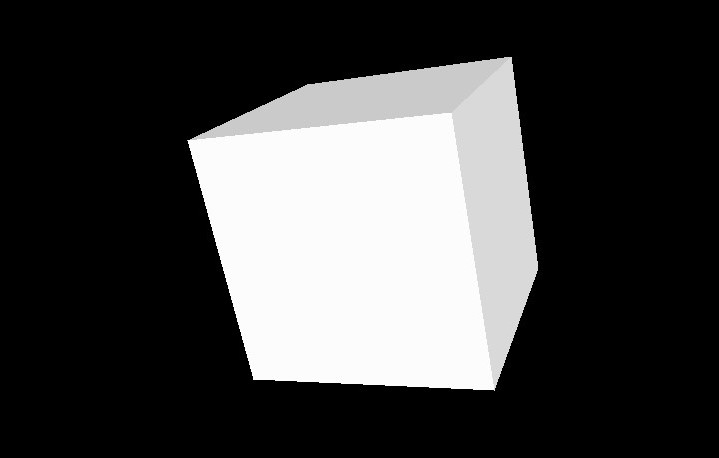
\includegraphics[scale=0.7]{cube}}
	\caption{Куб}
	\label{fig:cube}
\end{figure}

\begin{figure}[H]
	\center{
\includegraphics[scale=0.7]{tetr}}
	\caption{Тетраэдр}
	\label{fig:tetr}
\end{figure}

\begin{figure}[H]
	\center{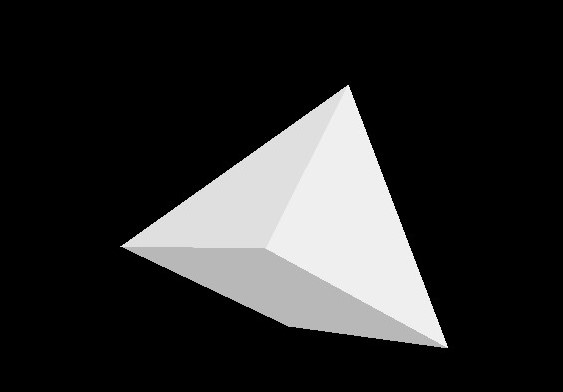
\includegraphics[scale=0.73]{pyram}}
	\caption{Пирамида}
	\label{fig:pyram}
\end{figure}

\begin{figure}[H]
	\center{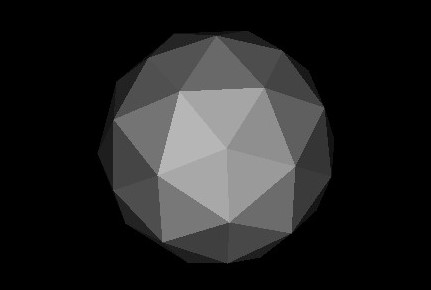
\includegraphics[scale=1.1]{isosphere}}
	\caption{Изосфера}
	\label{fig:isosphere}
\end{figure}

\begin{figure}[H]
	\center{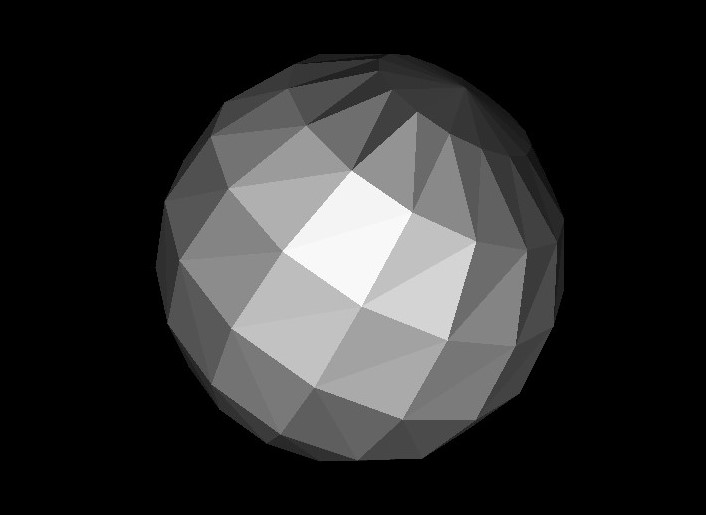
\includegraphics[scale=0.72]{sphere}}
	\caption{Сфера}
	\label{fig:sphere}
\end{figure}

\begin{figure}[H]
	\center{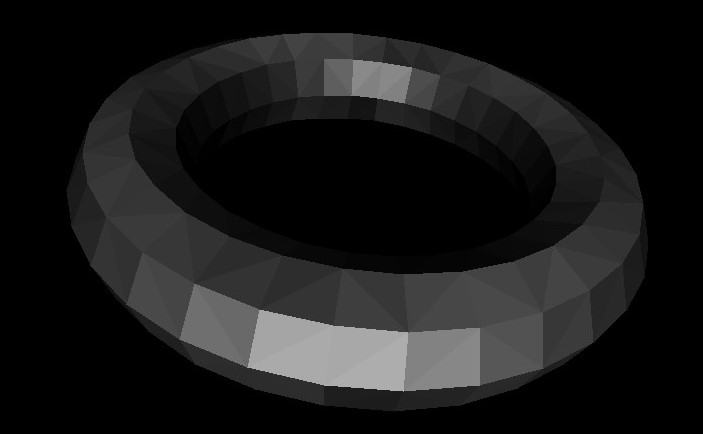
\includegraphics[scale=0.705]{torus}}
	\caption{Тор}
	\label{fig:torus}
\end{figure}

\begin{figure}[H]
	\center{
\includegraphics[scale=0.7]{cyllinder}}
	\caption{Циллиндр}
	\label{fig:cyllinder}
\end{figure}

\begin{figure}[H]
	\center{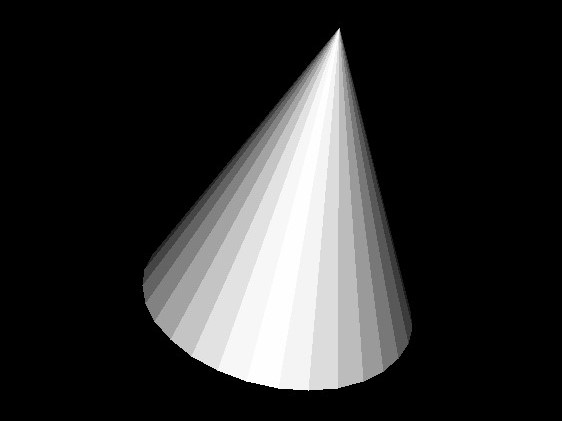
\includegraphics[scale=0.72]{cone}}
	\caption{Конус}
	\label{fig:cone}
\end{figure}
